\documentclass[11pt]{article}
\usepackage[margin=1in]{geometry}
\usepackage[T1]{fontenc}
\usepackage{lmodern}
\usepackage{amsmath,amssymb}
\usepackage{booktabs}
\usepackage{siunitx}
\usepackage{graphicx}
\usepackage{xcolor}
\usepackage[numbers,sort&compress]{natbib}
\usepackage{hyperref}
\usepackage{cleveref}
\usepackage{caption}
\usepackage{microtype}
\emergencystretch=3em
\captionsetup{font=small}
\hypersetup{colorlinks=true,linkcolor=blue!50!black,citecolor=blue!50!black,urlcolor=blue!50!black}

\newif\ifprovisional
\newif\ifcpprovisional
% GENERATED by figures/make_figures.py from results/*.json -- do not edit.
% benchmark source: dev-provisional.json
\provisionaltrue
\newcommand{\benchSource}{dev-provisional.json}
\newcommand{\benchDate}{2026-10-09}
\newcommand{\gpuName}{NVIDIA GeForce RTX 3070 Laptop GPU}
\newcommand{\driverVersion}{595.91.07}
\newcommand{\torchVersion}{2.7.0+cu126}
\newcommand{\tritonVersion}{3.3.0}
\newcommand{\warpVersion}{1.18.0}
\newcommand{\cupyVersion}{13.5.1}
\newcommand{\numbaVersion}{0.68.0}
\newcommand{\pythonVersion}{3.13.2}
\newcommand{\numpyVersion}{2.5.3}
\newcommand{\copyBW}{361}
\newcommand{\specBW}{448}
\newcommand{\measuredCopyBW}{163}
\newcommand{\rooflineFP}{45.1}
\newcommand{\rooflineHalf}{90.2}
\newcommand{\nRuns}{184}
\newcommand{\sizeTwoD}{8192^2}
\newcommand{\bestSingleTwoDVariant}{cupy-cuda-c/ymarch}
\newcommand{\bestSingleTwoDGLUPS}{32.7}
\newcommand{\bestSingleTwoDBW}{262}
\newcommand{\bestSingleTwoDPctCopy}{72}
\newcommand{\bestSingleTwoDPctSpec}{58}
\newcommand{\bestSingleTwoDMin}{32.4}
\newcommand{\bestSingleTwoDMax}{32.8}
\newcommand{\bestTBTwoDVariant}{cupy-cuda-c/tb8}
\newcommand{\bestTBTwoDGLUPS}{120.1}
\newcommand{\bestTBTwoDBW}{120}
\newcommand{\bestTBTwoDPctCopy}{33}
\newcommand{\bestTBTwoDPctSpec}{27}
\newcommand{\bestTBTwoDMin}{112.4}
\newcommand{\bestTBTwoDMax}{122.9}
\newcommand{\bestLowTwoDVariant}{cupy-cuda-c/naive-bf16}
\newcommand{\bestLowTwoDGLUPS}{53.5}
\newcommand{\bestLowTwoDBW}{214}
\newcommand{\bestLowTwoDPctCopy}{59}
\newcommand{\bestLowTwoDPctSpec}{48}
\newcommand{\bestLowTwoDMin}{52.5}
\newcommand{\bestLowTwoDMax}{56.6}
\newcommand{\bestTBTwoDK}{8}
\newcommand{\bestTBTwoDEquiv}{961}
\newcommand{\bestTBTwoDOverRoof}{2.66}
\newcommand{\bestTBTwoDHaloBW}{145}
\newcommand{\bestTBTwoDHaloBytes}{1.21}
\newcommand{\numpyTwoDGLUPS}{0.646}
\newcommand{\numpyTwoDSize}{512^2}
\newcommand{\speedupNumpyTwoD}{47}
\newcommand{\sizeThreeD}{320^3}
\newcommand{\bestSingleThreeDVariant}{triton/zmarch}
\newcommand{\bestSingleThreeDGLUPS}{18.5}
\newcommand{\bestSingleThreeDBW}{148}
\newcommand{\bestSingleThreeDPctCopy}{41}
\newcommand{\bestSingleThreeDPctSpec}{33}
\newcommand{\bestSingleThreeDMin}{18.5}
\newcommand{\bestSingleThreeDMax}{18.7}
\newcommand{\bestTBThreeDVariant}{cupy-cuda-c/tb3}
\newcommand{\bestTBThreeDGLUPS}{22.5}
\newcommand{\bestTBThreeDBW}{60}
\newcommand{\bestTBThreeDPctCopy}{17}
\newcommand{\bestTBThreeDPctSpec}{13}
\newcommand{\bestTBThreeDMin}{22.4}
\newcommand{\bestTBThreeDMax}{22.5}
\newcommand{\bestLowThreeDVariant}{triton/zmarch-fp16}
\newcommand{\bestLowThreeDGLUPS}{36.9}
\newcommand{\bestLowThreeDBW}{148}
\newcommand{\bestLowThreeDPctCopy}{41}
\newcommand{\bestLowThreeDPctSpec}{33}
\newcommand{\bestLowThreeDMin}{35.1}
\newcommand{\bestLowThreeDMax}{40.7}
\newcommand{\bestTBThreeDK}{3}
\newcommand{\bestTBThreeDEquiv}{180}
\newcommand{\bestTBThreeDOverRoof}{0.50}
\newcommand{\bestTBThreeDHaloBW}{80}
\newcommand{\bestTBThreeDHaloBytes}{3.54}
\newcommand{\numpyThreeDGLUPS}{0.438}
\newcommand{\numpyThreeDSize}{64^3}
\newcommand{\speedupNumpyThreeD}{71}
\newcommand{\perfTableRows}{2D & \texttt{triton} & \texttt{tile} & fp32 & 1 & 19.69 & 8 & 158 & 44 & 35 & -- \\
2D & \texttt{triton} & \texttt{tile-bf16} & bfp16 & 1 & 27.50 & 4 & 110 & 30 & 25 & -- \\
2D & \texttt{triton} & \texttt{tile-fp16} & fp16 & 1 & 50.74 & 4 & 203 & 56 & 45 & -- \\
2D & \texttt{warp} & \texttt{naive} & fp32 & 1 & 15.36 & 8 & 123 & 34 & 27 & -- \\
2D & \texttt{numba} & \texttt{naive} & fp32 & 1 & 13.14 & 8 & 105 & 29 & 23 & -- \\
2D & \texttt{cupy-cuda-c} & \texttt{naive} & fp32 & 1 & 19.10 & 8 & 153 & 42 & 34 & -- \\
2D & \texttt{cupy-cuda-c} & \texttt{naive-bf16} & bfp16 & 1 & 53.52 & 4 & 214 & 59 & 48 & -- \\
2D & \texttt{cupy-cuda-c} & \texttt{naive-fp16} & fp16 & 1 & 50.43 & 4 & 202 & 56 & 45 & -- \\
2D & \texttt{cupy-cuda-c} & \texttt{ymarch} & fp32 & 1 & 32.72 & 8 & 262 & 72 & 58 & -- \\
2D & \texttt{cupy-cuda-c} & \texttt{tb2} & fp32 & 2 & 74.60 & 4 & 298 & 83 & 67 & 597 \\
2D & \texttt{cupy-cuda-c} & \texttt{tb3} & fp32 & 3 & 89.94 & 2.7 & 240 & 66 & 54 & 720 \\
2D & \texttt{cupy-cuda-c} & \texttt{tb4} & fp32 & 4 & 115.42 & 2 & 231 & 64 & 52 & 923 \\
2D & \texttt{cupy-cuda-c} & \texttt{tb8} & fp32 & 8 & 120.13 & 1 & 120 & 33 & 27 & 961 \\
2D & \texttt{cupy-cuda-c} & \texttt{tb4-fp16} & fp16 & 4 & 146.16 & 1 & 146 & 40 & 33 & 585 \\
\midrule
3D & \texttt{torch-eager} & \texttt{slicing} & fp32 & 1 & 1.72 & 8 & 14 & 4 & 3 & -- \\
3D & \texttt{torch-compile} & \texttt{inductor} & fp32 & 1 & 15.60 & 8 & 125 & 35 & 28 & -- \\
3D & \texttt{triton} & \texttt{tile} & fp32 & 1 & 16.63 & 8 & 133 & 37 & 30 & -- \\
3D & \texttt{triton} & \texttt{tile-bf16} & bfp16 & 1 & 25.97 & 4 & 104 & 29 & 23 & -- \\
3D & \texttt{triton} & \texttt{tile-fp16} & fp16 & 1 & 27.83 & 4 & 111 & 31 & 25 & -- \\
3D & \texttt{triton} & \texttt{zmarch} & fp32 & 1 & 18.48 & 8 & 148 & 41 & 33 & -- \\
3D & \texttt{triton} & \texttt{zmarch-bf16} & bfp16 & 1 & 19.76 & 4 & 79 & 22 & 18 & -- \\
3D & \texttt{triton} & \texttt{zmarch-fp16} & fp16 & 1 & 36.95 & 4 & 148 & 41 & 33 & -- \\
3D & \texttt{warp} & \texttt{naive} & fp32 & 1 & 5.36 & 8 & 43 & 12 & 10 & -- \\
3D & \texttt{warp} & \texttt{zmarch} & fp32 & 1 & 9.39 & 8 & 75 & 21 & 17 & -- \\
3D & \texttt{numba} & \texttt{naive} & fp32 & 1 & 6.23 & 8 & 50 & 14 & 11 & -- \\
3D & \texttt{numba} & \texttt{zmarch} & fp32 & 1 & 9.50 & 8 & 76 & 21 & 17 & -- \\
3D & \texttt{cupy-cuda-c} & \texttt{naive} & fp32 & 1 & 10.12 & 8 & 81 & 22 & 18 & -- \\
3D & \texttt{cupy-cuda-c} & \texttt{naive-bf16} & bfp16 & 1 & 13.14 & 4 & 53 & 15 & 12 & -- \\
3D & \texttt{cupy-cuda-c} & \texttt{naive-fp16} & fp16 & 1 & 13.94 & 4 & 56 & 15 & 12 & -- \\
3D & \texttt{cupy-cuda-c} & \texttt{zmarch} & fp32 & 1 & 9.43 & 8 & 75 & 21 & 17 & -- \\
3D & \texttt{cupy-cuda-c} & \texttt{tb2} & fp32 & 2 & 17.72 & 4 & 71 & 20 & 16 & 142 \\
3D & \texttt{cupy-cuda-c} & \texttt{tb3} & fp32 & 3 & 22.48 & 2.7 & 60 & 17 & 13 & 180 \\
3D & \texttt{cupy-cuda-c} & \texttt{tb4} & fp32 & 4 & 21.24 & 2 & 42 & 12 & 9 & 170 \\
3D & \texttt{cupy-cuda-c} & \texttt{tb4-fp16} & fp16 & 4 & 18.26 & 1 & 18 & 5 & 4 & 73 \\}
\newcommand{\spatialOrderTwoD}{1.97}
\newcommand{\spatialErrFinestTwoD}{9.9\times10^{-7}}
\newcommand{\spatialNFinestTwoD}{257}
\newcommand{\spatialOrderThreeD}{1.99}
\newcommand{\spatialErrFinestThreeD}{2.4\times10^{-5}}
\newcommand{\spatialNFinestThreeD}{129}
\newcommand{\spatialOrderTwoDPer}{2.00}
\newcommand{\spatialErrFinestTwoDPer}{2.0\times10^{-6}}
\newcommand{\spatialNFinestTwoDPer}{512}
\newcommand{\spatialOrderThreeDPer}{2.08}
\newcommand{\spatialErrFinestThreeDPer}{1.2\times10^{-5}}
\newcommand{\spatialNFinestThreeDPer}{128}
\newcommand{\temporalOrderTwoD}{1.00}
\newcommand{\temporalNTwoD}{65}
\newcommand{\temporalOrderThreeD}{1.00}
\newcommand{\temporalNThreeD}{33}
\newcommand{\laplaceOrderTwoD}{1.99}
\newcommand{\laplaceErrFinestTwoD}{1.7\times10^{-5}}
\newcommand{\laplaceOrderThreeD}{1.98}
\newcommand{\laplaceErrFinestThreeD}{1.1\times10^{-4}}
\newcommand{\poissonOrderTwoD}{2.00}
\newcommand{\poissonErrFinestTwoD}{2.0\times10^{-4}}
\newcommand{\poissonOrderThreeD}{2.01}
\newcommand{\poissonErrFinestThreeD}{8.0\times10^{-4}}
\newcommand{\quadErrTwoD}{6.7\times10^{-15}}
\newcommand{\quadErrThreeD}{5.3\times10^{-15}}
\newcommand{\fpVariant}{torch-eager/slicing}
\newcommand{\nCross}{76}
\newcommand{\nCrossPass}{76}
\newcommand{\nVariants}{23}
\newcommand{\maxCrossErrFP}{5.1\times10^{-7}}
\newcommand{\maxCrossErrHalf}{8.9\times10^{-4}}
\newcommand{\maxCrossErrBF}{7.1\times10^{-3}}
\newcommand{\nBitwise}{6}
\newcommand{\fourierErrTwoD}{5.9\times10^{-6}}
\newcommand{\fourierDiscErrTwoD}{9.4\times10^{-6}}
\newcommand{\fourierNTwoD}{257}
\newcommand{\fourierStepsTwoD}{6554}
\newcommand{\fourierErrHalfTwoD}{2.2\times10^{-1}}
\newcommand{\fourierErrBFTwoD}{2.2\times10^{-1}}
\newcommand{\fourierErrTBHalfTwoD}{2.2\times10^{-1}}
\newcommand{\fourierErrThreeD}{6.0\times10^{-5}}
\newcommand{\fourierDiscErrThreeD}{1.2\times10^{-5}}
\newcommand{\fourierNThreeD}{65}
\newcommand{\fourierStepsThreeD}{410}
\newcommand{\fourierErrHalfThreeD}{7.3\times10^{-2}}
\newcommand{\fourierErrBFThreeD}{3.5\times10^{-1}}
\newcommand{\fourierErrTBHalfThreeD}{7.8\times10^{-4}}

% Fallbacks so the paper always builds; real values come from results.tex (generated).
\providecommand{\bestTBTwoDHaloBW}{n/a}\providecommand{\bestTBThreeDHaloBW}{n/a}
\providecommand{\bestTBTwoDHaloBytes}{n/a}\providecommand{\bestTBThreeDHaloBytes}{n/a}
\providecommand{\speedupNumpyTwoD}{n/a}\providecommand{\speedupNumpyThreeD}{n/a}
\providecommand{\maxCrossErrFP}{n/a}\providecommand{\maxCrossErrHalf}{n/a}
\providecommand{\maxCrossErrBF}{n/a}

\newcommand{\GLUPS}{\,GLUPS}
\newcommand{\code}[1]{\texttt{#1}}

\title{Stencils at the Roofline from Python:\\ the Heat Equation and Jacobi Iteration on a
Laptop GPU, and How Temporal Blocking Moves the Roof}
\author{Walid Hemati\\ \small Independent researcher}
\date{}

\begin{document}
\maketitle

\ifprovisional
\begin{center}
\fcolorbox{red!70!black}{red!8}{\parbox{0.92\linewidth}{\centering\bfseries\color{red!60!black}
PROVISIONAL NUMBERS. The performance figures in this version come from
\texttt{results/\benchSource}, measured during development on a GPU shared with other jobs.
They will be replaced by the serial, idle-GPU run of \texttt{bench/run.py --full}.}}
\end{center}
\fi

\begin{abstract}
The explicit heat equation with the 7-point (3D) or 5-point (2D) stencil, and the Jacobi
iteration that shares its update, are the textbook memory-bound kernels: about one floating
point operation per byte of DRAM traffic. We use them to test a simple claim: Python code on a
GPU reaches the same \emph{hardware efficiency} as hand-written CUDA C. One package,
\code{pyheat3d}, implements the update in NumPy, PyTorch eager and \code{torch.compile},
Triton, NVIDIA Warp, Numba-CUDA and hand-written CUDA C compiled at run time through CuPy, all
behind one interface and validated against analytic solutions (second order in space, first
order in time, to the expected rates) and against a NumPy oracle. On an RTX~3070 Laptop GPU the
best single-step kernel reaches \bestSingleThreeDGLUPS\GLUPS{} on a $\sizeThreeD$ grid, which is
\bestSingleThreeDPctCopy\% of the measured \copyBW\,GB/s copy bandwidth under a minimal
8-byte-per-update traffic model. We then add temporal blocking, which fuses $k$ time steps
into one DRAM pass. This does not beat the hardware. It lowers the traffic per update $k$-fold
and so raises the per-step roofline by the same factor. With it the CUDA C variant reaches
\bestTBThreeDGLUPS\GLUPS{} in 3D (\bestTBThreeDOverRoof$\times$ the single-step roofline) and
\bestTBTwoDGLUPS\GLUPS{} in 2D. We report both lattice updates per second and the estimated DRAM
traffic behind them.
\end{abstract}

\section{Introduction}
Stencil codes sweep a grid and update each site from a few neighbours. They do very little
arithmetic per byte moved, so on modern hardware their speed is set by memory bandwidth, not by
floating point throughput. The roofline model~\cite{williams2009roofline} makes this exact: a
kernel with arithmetic intensity $I$ (FLOP/byte) cannot exceed $\min(P, I\cdot B)$, where $P$
is peak compute and $B$ peak bandwidth. For the explicit heat equation in single precision,
$I\approx 1$ FLOP/byte and the bandwidth term dominates by more than an order of magnitude.

That makes the heat equation a fair test for high-level languages. There is no algorithmic
headroom to hide behind and no tensor core to borrow. Whatever reaches the copy bandwidth has
done the job, whether it is Python or C. This paper asks how close each mainstream Python GPU
route gets, what it costs in code, and what happens when the algorithm itself changes the
roof.

\paragraph{Contributions.}
\begin{itemize}
\item An optimisation ladder for the same stencil in seven backends (NumPy, PyTorch eager,
  \code{torch.compile}, Triton, Warp, Numba-CUDA, CUDA C via CuPy/NVRTC), each as a variant in a
  common registry with one interface, one test suite and one benchmark harness.
\item Validation that does not depend on any backend: the decaying Fourier mode against its
  continuous, semi-discrete and fully discrete exact solutions, Laplace and Poisson steady
  states, and \nCrossPass/\nCross{} cross-backend comparisons against a NumPy oracle.
\item A roofline analysis with a stated minimal traffic model. Every throughput is reported as
  lattice-site updates per second and as a percentage of the measured copy bandwidth
  (\copyBW\,GB/s) and of the specification (\specBW\,GB/s).
\item Temporal-blocking kernels written from Python (3D: shared memory plus warp shuffles with
  register blocking; 2D: warp-synchronous, no shared memory). They exceed the single-step
  roofline, and we explain exactly why this is not the same as exceeding the hardware.
\item A same-GPU head-to-head with two established stencil codes, the pystencils code
  generator and AN5D's temporal-blocking CUDA, on the identical update.
\end{itemize}

\section{Background and related work}
\paragraph{Roofline.}
Williams, Waterman and Patterson~\cite{williams2009roofline} bound attainable performance by
peak compute and by bandwidth times operational intensity, where intensity counts bytes of
DRAM traffic. The bound depends on the \emph{traffic}, not on the FLOPs alone. Any
transformation that cuts traffic per unit of work raises the ceiling for that work.

\paragraph{Stencil optimisation.}
Datta et al.~\cite{datta2008stencil} auto-tuned 7-point stencils across multicore
architectures and showed they are bandwidth bound once cache blocking removes redundant
loads. On GPUs, Micikevicius~\cite{micikevicius2009fd} introduced the now standard 2.5D scheme:
a thread block holds an $xy$ tile in shared memory and marches along $z$, keeping the $z$
neighbours in registers. Nguyen et al.~\cite{nguyen2010blocking} combined 2.5D spatial
blocking with temporal blocking (``3.5D'') on CPUs and GPUs. Holewinski, Pouchet and
Sadayappan~\cite{holewinski2012stencil} generated GPU stencil code with overlapped tiling,
recomputing halos redundantly instead of synchronising between blocks. pystencils, the code
generator behind waLBerla~\cite{bauer2019pystencils,bauer2021walberla}, turns symbolic stencil
updates written in Python into CPU and GPU kernels.

\paragraph{Temporal blocking.}
Wonnacott's time skewing~\cite{wonnacott2000timeskewing} reorders the iteration space so that
several time steps run on data still in cache. That removes the bandwidth limit in exchange for
more work per byte. Wellein et al.~\cite{wellein2009temporal} pipelined successive time steps
across cores sharing a cache (wavefront parallelisation). Malas et al.~\cite{malas2015diamond}
used diamond tiling with multicore wavefronts. Our temporally blocked kernels are a GPU form of
the wavefront idea: a thread block streams through $z$ and $k$ pipeline stages advance the same
columns by $k$ time levels, using overlapped (redundant) halos as
in~\cite{holewinski2012stencil}. AN5D~\cite{matsumura2020an5d} generates GPU code with
temporal blocking degrees up to 10 from C loop nests, guided by a performance model.

\paragraph{Python on GPUs.}
NumPy~\cite{harris2020numpy} defines the array model the others imitate. PyTorch~2's
\code{torch.compile}~\cite{ansel2024pytorch2} captures Python into a graph and generates fused
Triton kernels. Triton~\cite{tillet2019triton} lets one write block-level kernels in Python and
leaves intra-block scheduling to the compiler. Warp~\cite{macklin2022warp} and
Numba~\cite{lam2015numba} compile SIMT kernels written in a Python subset. CuPy~\cite{okuta2017cupy}
provides NumPy-compatible arrays and runtime compilation of CUDA C through NVRTC. We use the
last route as our ``hand-written CUDA C'' reference: the kernels are compiled at run time by NVRTC, so the
package needs no CUDA toolkit or \code{nvcc} at install time.

\section{Method}
\subsection{Physics and numerics}
We solve $u_t=\alpha\nabla^2u$ on the unit square or cube with forward Euler in time and
second-order central differences in space (FTCS). With uniform spacing $h$ and the mesh Fourier
number $r=\alpha\Delta t/h^2$ the update is
\begin{equation}
u'_c = (1-2dr)\,u_c + r\,S_c,\qquad
S_c=\big[(u_{x-1}+u_{x+1})+(u_{y-1}+u_{y+1})\big]+(u_{z-1}+u_{z+1}),
\label{eq:update}
\end{equation}
where $d\in\{2,3\}$. The von Neumann limit is $r\le 1/(2d)$, which the code enforces. Every
backend uses the same bracketing of $S_c$, so they differ at most by fused multiply-add
contraction. Dirichlet problems keep a fixed boundary layer that no kernel writes; periodic
problems wrap indices. The Jacobi iteration for $\nabla^2u=f$ is the same update with
$c_0=0$, $c_1=1/(2d)$ and an additive term $-h^2f/(2d)$. All kernels are written for the generic
$u'=c_0u+c_1S$ and run both modes.

\subsection{Reference solutions}
For the mode $u_0=\prod_i\sin(\kappa x_i)$ ($\kappa=\pi$ Dirichlet, $2\pi$ periodic) three exact
references exist:
(i) the PDE solution $e^{-\alpha d\kappa^2 t}u_0$;
(ii) the semi-discrete (exact-in-time) solution $e^{-\alpha\lambda_h t}u_0$ with
$\lambda_h=4d\sin^2(\kappa h/2)/h^2$; and
(iii) the fully discrete solution $g^n u_0$ with $g=1-4dr\sin^2(\kappa h/2)$, which FTCS must
reproduce to round-off. Error against (i) at fixed $r$ measures the combined
$\mathcal{O}(h^2)+\mathcal{O}(\Delta t)=\mathcal{O}(h^2)$ error. Error against (ii) on a fixed
grid isolates the first-order temporal error. Error against (iii) is a pure implementation
check. We avoid $r=1/(6d)$, where the leading space and time error terms cancel.

For Laplace we use $\sin(\pi x)\sinh(\pi y)/\sinh\pi$ (2D) and
$\sin(\pi x)\sin(\pi y)\sinh(\sqrt2\pi z)/\sinh(\sqrt2\pi)$ (3D), and quadratic harmonic
functions on which the discrete Laplacian is exact. For Poisson we use a manufactured solution
$u=\prod\sin(\pi x_i)$.

\section{Implementation}
\subsection{One interface, a registry of variants}
Each variant is a \code{Stepper} that owns two device buffers and exposes \code{step(n)},
\code{get()} and \code{synchronize()}. A registry entry records backend, dimensionality,
storage type and $k$, the number of time steps fused per DRAM pass. Tests, validation and
benchmarks loop over the registry. Variants whose package or GPU is missing are skipped.
\Cref{tab:ladder} lists the ladder.

\begin{table}[t]
\centering\small
\caption{The optimisation ladder. $k$: time steps per DRAM pass.}
\label{tab:ladder}
\begin{tabular}{@{}lllp{7.4cm}@{}}
\toprule
backend & variant & $k$ & idea \\
\midrule
numpy & slicing & 1 & vectorised slices, CPU; correctness oracle \\
torch-eager & slicing & 1 & same slices on the GPU; one kernel per operator \\
torch-compile & inductor & 1 & the same Python traced and fused into one Triton kernel \\
triton & tile(-fp16/-bf16) & 1 & 2D/3D tiles, neighbours as shifted masked loads \\
triton & zmarch(-fp16/-bf16) & 1 & 3D: $xy$ tile marches in $z$ with a register queue \\
warp, numba & naive, zmarch & 1 & one thread per site; per-thread $z$ column with register queue \\
cupy-cuda-c & naive(-fp16/-bf16) & 1 & one thread per site (several per thread for 2-byte types) \\
cupy-cuda-c & zmarch, ymarch & 1 & 2.5D: shared-memory plane + register queue~\cite{micikevicius2009fd} \\
cupy-cuda-c & tb2, tb3, tb4, tb8 & $k$ & temporal blocking (wavefront, overlapped halos) \\
cupy-cuda-c & tb4-fp16 & 4 & temporal blocking with fp16 storage \\
\bottomrule
\end{tabular}
\end{table}

\subsection{Traffic model and roofline}
\label{sec:traffic}
We use the \emph{minimal} traffic model: a sweep that advances the field by $k$ steps must read
each value once and write it once, so the DRAM traffic per lattice-site update is
\begin{equation}
B_{\text{upd}} = \frac{2\,b}{k},\qquad b=\text{bytes per stored value}.
\label{eq:traffic}
\end{equation}
That is 8\,B for fp32 single-step kernels and 4\,B for fp16/bf16 storage. Reported effective
bandwidth is $\text{LUPS}\times B_{\text{upd}}$. Halo re-reads and cache misses are not counted,
so this is a lower bound on true traffic; an inefficient kernel cannot inflate it. With the
measured \copyBW\,GB/s copy bandwidth the single-step fp32 roofline is
$\copyBW/8=\rooflineFP$\GLUPS{} and the 2-byte roofline is \rooflineHalf\GLUPS. The update needs
$2d+2$ FLOPs (\cref{eq:update}), so $I=1$ FLOP/byte in 3D: at least 25$\times$ below the ridge
point of this GPU.

\paragraph{What temporal blocking does to the roof.}
For a $k$-step kernel \cref{eq:traffic} gives $8/k$ bytes per fp32 update, so its roofline is
$k\cdot\rooflineFP$\GLUPS. A temporally blocked kernel that delivers more than \rooflineFP\GLUPS{}
has not moved data faster than the hardware allows. It moves $k$ times less data per update.
For these kernels we therefore report three numbers: the update rate; the DRAM traffic implied
by \cref{eq:traffic} (always below the copy bandwidth); and the ``single-step-equivalent
bandwidth'' $\text{LUPS}\times 8$\,B. The last one is \emph{not} a DRAM rate, only the
bandwidth a $k=1$ kernel would need to match the rate. For the CUDA C kernels we also give a
more realistic \emph{halo model} that adds the redundant halo reads of overlapped tiling
(\cref{sec:tb}), assuming no L2 reuse between blocks.

\subsection{Kernels}
\paragraph{Tiles, compiled expressions and naive SIMT.}
The Triton tile kernels load the centre tile and its four or six shifted neighbours as masked
loads. Reuse between neighbouring loads is left to L1/L2. \code{torch.compile} receives the
NumPy-style expression of \cref{eq:update} with slicing (Dirichlet) or \code{torch.roll}
(periodic) and lowers it to one fused kernel. Warp, Numba and the naive CUDA C kernels use one
thread per site. For 2-byte storage the CUDA C kernel handles several sites per thread, to keep
enough bytes in flight.

\paragraph{2.5D z-marching.}
Following~\cite{micikevicius2009fd}, the CUDA C \code{zmarch} kernel stages the current $z$
plane plus a one-site halo in shared memory and keeps the $z\pm1$ values in a register queue.
It prefetches the next plane one iteration ahead. The Triton, Warp and Numba \code{zmarch}
variants keep the register queue and leave $x/y$ reuse to the caches.

\paragraph{Temporal blocking.}
\label{sec:tb}
The 3D kernel assigns a $32\times T_y$ thread block to an extended $xy$ tile of
$32\times(T_yR)$ columns. Lane $x$ owns a column and each thread owns $R$ consecutive $y$ rows
(register blocking). The block streams through the planes of a $z$ chunk. At iteration $i_z$ it
loads level $t$ of plane $i_z$, and stage $s=1..k$ computes level $t+s$ of plane $i_z-s$ from a
register queue of level $t+s-1$. That is a wavefront in $(z,t)$, as in~\cite{wellein2009temporal},
mapped onto one thread block. The $x$ neighbours come from warp shuffles, the $y$ neighbours
from the thread's own registers, and only the first and last row of each thread pass through
shared memory, with one barrier per stage. The halo is recomputed redundantly (overlapped
tiling~\cite{holewinski2012stencil}). The valid region shrinks by one column per stage, and
only the central $(32-2k)\times(T_yR-2k)$ columns are stored, once per $k$ steps. The 2D kernel
is warp-synchronous: each warp owns an $x$ strip of $32R$ columns, with lane $l$ holding columns
$l, l+32, \dots$ so every load is coalesced. It marches along $y$ with no shared memory and no
barriers. The chunk length along the marching direction is chosen at run time so small grids
still fill the GPU. Intermediate levels never leave registers, so the fp32 kernels give the
same arithmetic as $k$ single steps and the fp16 kernel rounds to storage only once per $k$
steps.

All CUDA C kernels are one source file compiled by NVRTC with macros for storage type,
boundary condition, $k$ and tile shape. The Python side picks the launch configuration. The
backends together are about 1{,}400 lines of Python and CUDA C, comments included.

\section{Validation}
\Cref{fig:validation} summarises the studies. They run with the fp64-capable variant
\code{\fpVariant}, except panel (d). Against the PDE solution at fixed $r=0.1$ the observed
spatial order is \spatialOrderTwoD{} (2D) and \spatialOrderThreeD{} (3D) with Dirichlet walls,
and \spatialOrderTwoDPer{}/\spatialOrderThreeDPer{} on periodic grids. The finest 3D grid
($\spatialNFinestThreeD^3$) has relative error $\spatialErrFinestThreeD$. Against the
semi-discrete solution on a fixed grid the temporal order is \temporalOrderTwoD{} (2D,
$n=\temporalNTwoD$) and \temporalOrderThreeD{} (3D, $n=\temporalNThreeD$). The converged Jacobi
solutions converge to the smooth harmonic functions with order \laplaceOrderTwoD{} (2D) and
\laplaceOrderThreeD{} (3D). The manufactured Poisson problems converge with
\poissonOrderTwoD{} and \poissonOrderThreeD. On the quadratic harmonic function, where the
stencil is exact, Jacobi recovers the solution to $\quadErrThreeD$ (3D), which is round-off and
iteration tolerance only.

Every GPU variant reproduces the fully discrete FTCS solution of the Fourier mode to at most
$\fourierDiscErrThreeD$ in 3D (fp32, $\fourierNThreeD^3$, \fourierStepsThreeD{} steps), while
its error against the PDE is $\fourierErrThreeD$. Round-off is therefore far below
discretisation error. On random fields with both boundary conditions,
\nCrossPass{} of \nCross{} comparisons of \nVariants{} variants against the NumPy oracle pass.
The worst fp32 relative deviation is $\maxCrossErrFP$, which comes from FMA contraction only.
fp16 and bf16 variants are compared with a NumPy reference that applies the same storage
rounding after every DRAM pass (worst $\maxCrossErrHalf$ and $\maxCrossErrBF$). That makes the
test exact up to a few storage ulps.

Storage precision matters for physics: on the decaying mode the fp16 and bf16 single-step
variants reach $\fourierErrHalfThreeD$ and $\fourierErrBFThreeD$ against the PDE in 3D, against
$\fourierErrThreeD$ in fp32, because each step's small increment $r\nabla^2u$ is rounded to an
8- or 11-bit mantissa. Temporal blocking with fp16 storage rounds only every fourth step and
lands at $\fourierErrTBHalfThreeD$. Low-precision storage halves the roofline cost, but for
long diffusive runs bf16 is not accurate enough.

\begin{figure}[t]
\centering
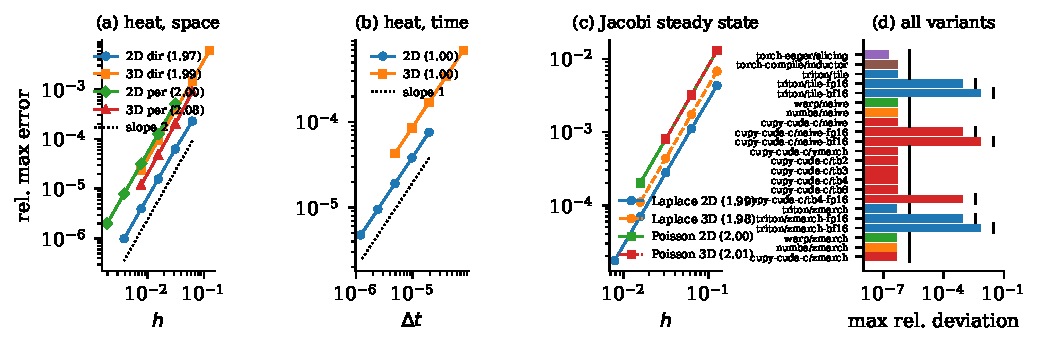
\includegraphics[width=\linewidth]{../figures/validation.pdf}
\caption{Validation. (a) Error against the exact PDE solution of a decaying sine mode at fixed
$r=0.1$ (2nd order). (b) Error against the semi-discrete solution on a fixed grid (1st order in
$\Delta t$). (c) Jacobi steady states for Laplace and Poisson. (d) Worst relative deviation of
every GPU variant from the (storage-emulating) NumPy reference; ticks mark the tolerance.
Observed orders in the legends.}
\label{fig:validation}
\end{figure}

\section{Performance}
All numbers come from \code{bench/run.py} (\texttt{results/\benchSource}, \nRuns{} runs,
\gpuName, driver \driverVersion, PyTorch \torchVersion, Triton \tritonVersion, Warp
\warpVersion, CuPy \cupyVersion, Numba \numbaVersion, Python \pythonVersion). Each run warms up
(including JIT compilation), synchronises the device around the timed region and reports the
median of five repeats, each long enough to be timed reliably, together with min and max.
Dirichlet heat mode at $r=0.9/(2d)$, fp32 unless stated.

\begin{figure}[t]
\centering
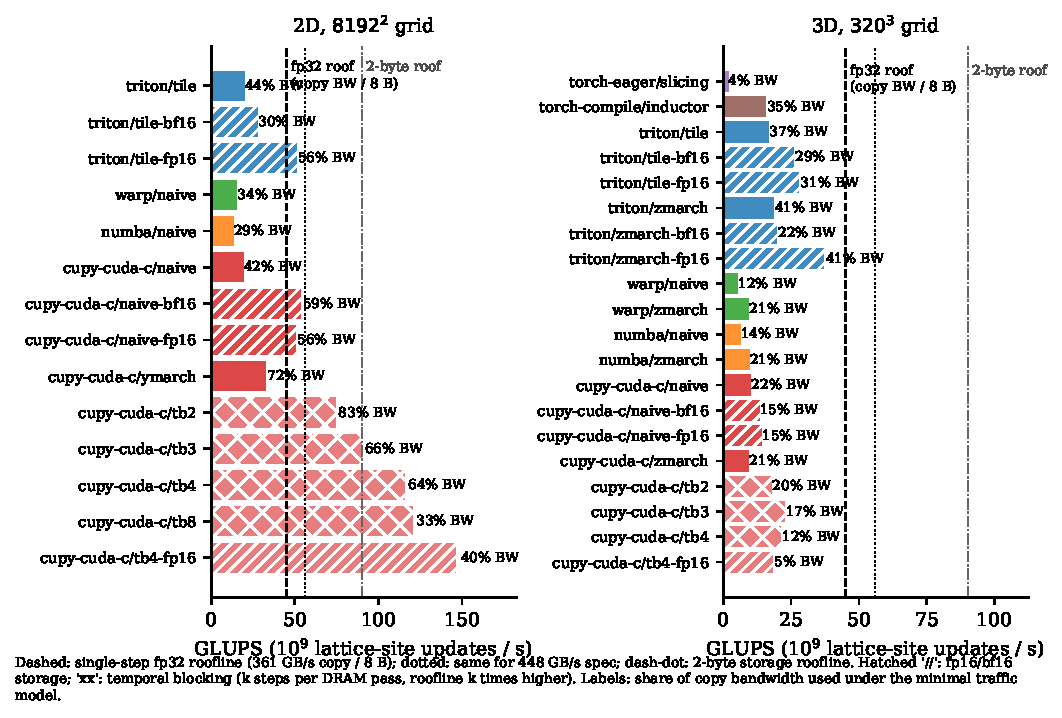
\includegraphics[width=\linewidth]{../figures/roofline.pdf}
\caption{Throughput of every variant at the largest benchmarked size, against the fp32
single-step roofline (dashed, copy bandwidth / 8\,B), the same at the specification bandwidth
(dotted) and the 2-byte roofline (dash-dot). Labels give the share of copy bandwidth used under
the minimal traffic model. Temporally blocked variants (``xx'') sit above the single-step roof
while using less bandwidth, because their roof is $k$ times higher.}
\label{fig:roofline}
\end{figure}

\paragraph{Single step: Python at the roof.}
In 3D ($\sizeThreeD$) the best single-step variant, \code{\bestSingleThreeDVariant}, runs at
\bestSingleThreeDGLUPS\GLUPS{} (min--max \bestSingleThreeDMin--\bestSingleThreeDMax). That
implies \bestSingleThreeDBW\,GB/s of DRAM traffic: \bestSingleThreeDPctCopy\% of the measured
copy bandwidth and \bestSingleThreeDPctSpec\% of the specification. In 2D ($\sizeTwoD$) the best
is \code{\bestSingleTwoDVariant} with \bestSingleTwoDGLUPS\GLUPS{}
(\bestSingleTwoDPctCopy\% of copy). \Cref{fig:roofline,tab:perf} show which Python routes reach
the level of the hand-written CUDA C (\pctCudaTwoD\% of copy in 2D, \pctCudaThreeD\% in 3D). In
2D, \code{torch.compile} (\pctCompileTwoD\%) and Triton (\pctTritonTwoD\%) do; the plain Warp
and Numba kernels stop at \pctWarpTwoD\% and \pctNumbaTwoD\%. In 3D the z-marching kernels in
Numba (\pctNumbaThreeD\%), Warp (\pctWarpThreeD\%) and Triton (\pctTritonThreeD\%) do, while
\code{torch.compile} reaches \pctCompileThreeD\%. Where they reach it, the Python routes differ
more in small-size launch overhead (\cref{fig:scaling}) than in large-size bandwidth. PyTorch eager is far below,
for a structural reason: each of its roughly ten operators is a separate pass over memory. The
same Python expression handed to \code{torch.compile} runs as one kernel. Against NumPy on the
16-core CPU the best GPU kernel is \speedupNumpyThreeD$\times$ faster in 3D at
$\numpyThreeDSize$.

\paragraph{Low-precision storage.}
fp16/bf16 storage halves $B_{\text{upd}}$. The best 2-byte single-step variant in 3D,
\code{\bestLowThreeDVariant}, reaches \bestLowThreeDGLUPS\GLUPS{}, that is
\bestLowThreeDBW\,GB/s or \bestLowThreeDPctCopy\% of copy bandwidth. 2-byte kernels need more
independent loads in flight per thread to saturate DRAM, so they sit further below their own
roof than fp32 kernels do below theirs.

\paragraph{Temporal blocking: a higher roof, not faster DRAM.}
The CUDA C kernel \code{\bestTBThreeDVariant} ($k=\bestTBThreeDK$) delivers
\bestTBThreeDGLUPS\GLUPS{} in 3D, \bestTBThreeDOverRoof$\times$ the single-step fp32 roofline.
Under the minimal model it moves \bestTBThreeDBW\,GB/s (\bestTBThreeDPctCopy\% of copy). With the
halo over-fetch of overlapped tiling the estimate is \bestTBThreeDHaloBW\,GB/s
(\bestTBThreeDHaloBytes\,B per update). A single-step kernel would need
\bestTBThreeDEquiv\,GB/s of DRAM bandwidth to match the rate (the specification is
\specBW\,GB/s). In 2D,
\code{\bestTBTwoDVariant} ($k=\bestTBTwoDK$) reaches \bestTBTwoDGLUPS\GLUPS{}
(\bestTBTwoDOverRoof$\times$ the single-step roof) while using \bestTBTwoDBW\,GB/s. The gain
saturates with $k$: redundant halo work grows as $(T-2k)^{-1}$ per tiled dimension, the
pipeline holds $3k$ values per site in registers, and in 3D every stage costs a barrier. At
large $k$ these kernels become instruction-bound rather than bandwidth-bound.
\Cref{fig:roofline-classic} shows the same data on the classic roofline. Temporal blocking
moves points to the right (higher intensity); it does not move them above the memory roof.

\ifdefined\cpMode
\subsection{Head-to-head with established stencil codes}
\label{sec:counterparts}
To check our kernels against code written by others, \code{bench/counterparts.py} runs two
established stencil codes on the same GPU, in the same session as our own variants, with the
same update (\cref{eq:update}, fp32, Dirichlet, $r=0.9/(2d)$).
\emph{pystencils}~\cite{bauer2019pystencils} (version \cpPystencilsVersion, CUDA target through
CuPy) is the Python counterpart of our single-step kernels. We run it as a user would
(\code{default}: runtime-sized fields, default block size) and tuned (\code{tuned}: shape fixed
at code generation, block size picked by timing five candidates).
\emph{AN5D}~\cite{matsumura2020an5d} is the temporal-blocking counterpart. Its generator needs
LLVM/Clang~3.4 and GCC~4.8, so we use the CUDA code it generated for the published artifact
(commit \code{\cpAnCommit}, 5-point \code{star2d1r} and 7-point \code{star3d1r}), substitute our
coefficients, and build it with \code{nvcc} \cpNvcc{} for sm\_86 with the artifact's flags. Its
configurations were tuned for P100/V100, not for this GPU; we report the best of the shipped
ones (\cpAnTwoDN{} in 2D and \cpAnThreeDN{} in 3D in this run) and keep AN5D's own timer. Before
timing, every counterpart matches our NumPy oracle after \cpVerifySteps{} steps on
$\cpVerifyTwoD^2$ and $\cpVerifyThreeD^3$ grids to $\cpVerifyErr$ (largest absolute deviation,
data in $[0,1)$), which is fp32 rounding: the codes differ only in summation order.
\ifcpprovisional{\color{red!60!black} These numbers come from a short run on smaller grids
($\cpSizeTwoD$, $\cpSizeThreeD$) on a GPU shared with other jobs and are provisional; the
idle-GPU run \code{bench/counterparts.py --full} at $16384^2$ and $512^3$ replaces them.}\fi

\begin{figure}[t]
\centering
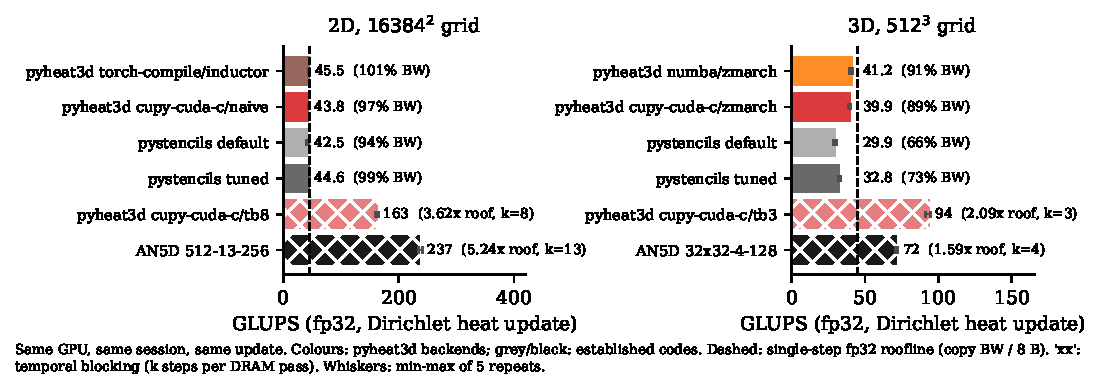
\includegraphics[width=\linewidth]{../figures/counterparts.pdf}
\caption{Head-to-head on one GPU in one session: our best Python-DSL and CUDA C single-step
kernels, pystencils (grey), our best temporal-blocking kernel and AN5D's best shipped
configuration (black). Dashed: single-step fp32 roofline.}
\label{fig:counterparts}
\end{figure}

For a single step (\cref{fig:counterparts}), tuned pystencils reaches \cpPsTunedTwoDGLUPS\GLUPS{}
in 2D (\cpPsTunedTwoDPct\% of copy) and \cpPsTunedThreeDGLUPS\GLUPS{} in 3D
(\cpPsTunedThreeDPct\%), and \cpPsDefaultTwoDGLUPS{} and \cpPsDefaultThreeDGLUPS\GLUPS{} with its
defaults. Our best Python-DSL kernels reach \cpPyDslTwoDGLUPS{} (\code{\cpPyDslTwoDVariant}) and
\cpPyDslThreeDGLUPS\GLUPS{} (\code{\cpPyDslThreeDVariant}). The faster is \cpSingleFasterTwoD{}
in 2D, by $\cpSingleRatioTwoD\times$, and \cpSingleFasterThreeD{} in 3D, by
$\cpSingleRatioThreeD\times$. pystencils generates one thread per site; in 3D that is the
structure of our naive kernels, without the $z$-marching schedule. With temporal blocking, AN5D's
\code{\cpAnTwoDVariant} ($b_T=\cpAnTwoDK$) reaches \cpAnTwoDGLUPS\GLUPS{}
($\cpAnTwoDOverRoof\times$ the single-step roof) and \code{\cpAnThreeDVariant}
($b_T=\cpAnThreeDK$) \cpAnThreeDGLUPS\GLUPS{} ($\cpAnThreeDOverRoof\times$), against
\cpPyTBTwoDGLUPS{} (\code{\cpPyTBTwoDVariant}) and \cpPyTBThreeDGLUPS\GLUPS{}
(\code{\cpPyTBThreeDVariant}) for ours. The faster is \cpTBFasterTwoD{} in 2D, by
$\cpTBRatioTwoD\times$, and \cpTBFasterThreeD{} in 3D, by $\cpTBRatioThreeD\times$. AN5D fuses
up to ten steps per pass in 2D where our kernels stop at eight, and was designed to keep
register and shared-memory pressure low at such depths~\cite{matsumura2020an5d}. This rung of
our ladder is CUDA C launched from Python, so it compares hand-written with generated CUDA, not
Python with C.
\fi

\begin{figure}[t]
\centering
\begin{minipage}[t]{0.42\linewidth}\vspace{0pt}
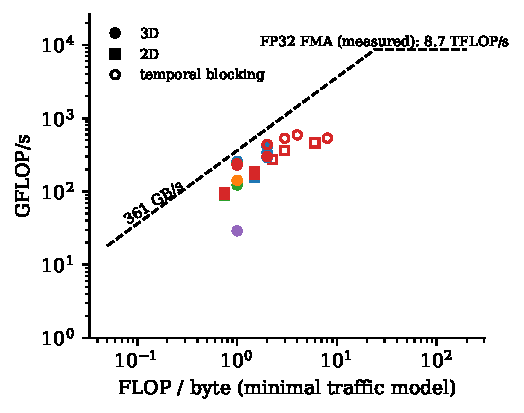
\includegraphics[width=\linewidth]{../figures/roofline_classic.pdf}
\caption{Classic roofline. Intensity uses the minimal traffic model, so temporally blocked
kernels (open symbols) sit $k$ times further right.}
\label{fig:roofline-classic}
\end{minipage}\hfill
\begin{minipage}[t]{0.55\linewidth}\vspace{0pt}
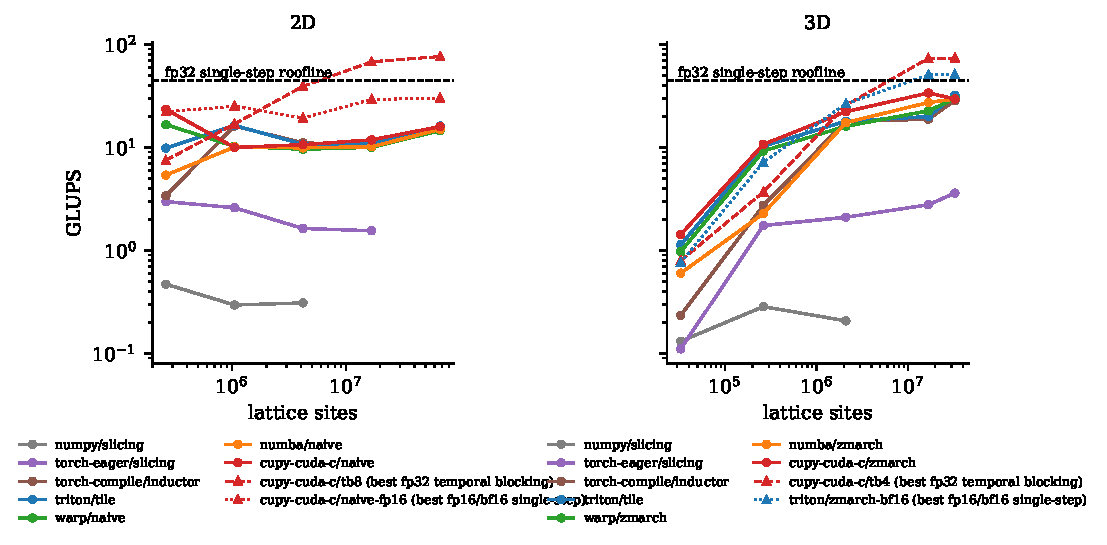
\includegraphics[width=\linewidth]{../figures/scaling.pdf}
\caption{Throughput against problem size for the best fp32 single-step variant of each
backend, the best temporally blocked and the best 2-byte variant. Small grids are bound by
Python launch overhead and fit in the 4\,MB L2.}
\label{fig:scaling}
\end{minipage}
\end{figure}

\begin{table}[t]
\centering\scriptsize
\caption{All variants at the largest benchmarked size. GB/s and \% use the minimal traffic
model $B_{\text{upd}}=2b/k$. ``equiv.'': single-step-equivalent bandwidth $\text{LUPS}\times
8$\,B (not a DRAM rate).}
\label{tab:perf}
\setlength{\tabcolsep}{4pt}
\begin{tabular}{@{}lllrrrrrrrr@{}}
\toprule
& backend & variant & store & $k$ & GLUPS & B/upd & GB/s & \% copy & \% spec & equiv. \\
\midrule
\perfTableRows
\\ \bottomrule
\end{tabular}
\end{table}

\section{Discussion}
\paragraph{Why Python gets there.}
A memory-bound kernel needs three things: coalesced access, enough bytes in flight, and no
redundant passes. Triton's block model gives the first two by construction. \code{torch.compile}
gives the third by fusion. Warp and Numba expose plain SIMT: in 3D, once each thread marches
through $z$ with coalesced rows, they match CUDA C; their simple 2D kernels, without that
schedule, stay at \pctWarpTwoD--\pctNumbaTwoD\%. Inductor's generic 3D schedule
(\pctCompileThreeD\%) shows the same point from the other side: the schedule matters, not the
language. The
interpreter costs microseconds per launch and nothing per byte. What Python does \emph{not} give
for free are the explicit shared-memory and warp-shuffle schedules that temporal blocking needs.
Triton deliberately hides them. For that rung we wrote CUDA C, but compiled and launched it from
Python.

\paragraph{Threats to validity.}
(i) One laptop GPU: absolute numbers do not transfer, but percentages of the measured copy
bandwidth should transfer better.
(ii) Laptop GPUs throttle with temperature and power. Each run records SM clock, temperature
and power, and the final benchmark runs serially on an idle GPU.
\ifprovisional (iii) The numbers in this version were measured while other jobs shared the GPU
and are pessimistic: the copy bandwidth measured at the start of that run was only
\measuredCopyBW\,GB/s instead of \copyBW\,GB/s. \fi
(iv) The CUDA C reference is compiled by NVRTC, not \code{nvcc}. Both use the same NVVM and
ptxas pipeline,
but default flags differ.
(v) The minimal traffic model ignores halo re-reads, and on small grids part of the working set
stays in the 4\,MB L2. Effective bandwidths for small grids can therefore exceed what DRAM
alone could deliver. We base claims on the largest grids.
(vi) Tile shapes were tuned briefly on a shared GPU and are unlikely to be optimal.

\section{Conclusion}
For the canonical memory-bound stencil, Python reaches the hardware ceiling: in 2D
\code{torch.compile} and Triton, in 3D z-marching kernels in Numba, Warp and Triton run at the
level of hand-written CUDA C, close to the copy bandwidth. Where a Python route falls short, it
lacks a schedule, not a language feature. Beyond that ceiling only algorithmic change helps. Temporal blocking raises the update
rate above the single-step roofline by cutting traffic per update. We report it as a change of
roofline, with its traffic, not as a victory over the hardware.

\section*{Code availability}
Code, benchmark JSON, figure scripts and this paper:
\url{https://github.com/walidhemati/pyheat3d} (MIT licence). \code{bench/run.py --full}
regenerates every number, and \code{figures/make\_figures.py} regenerates every figure and the
macro file this paper is typeset from.

\bibliographystyle{unsrtnat}
\bibliography{references}

\end{document}
